\chapter{Self-diffusion and structural properties of confined fluids in dynamic coexistence\label{chap7}}

\section{Introduction}

The thermodynamics and molecular dynamics of gases, liquids, and solids confined to small volumes can differ significantly from those of the bulk \cite{Pawlow:1909,Hill:1963}. The confinement of a fluid in a region few times the particle diameter induces density layering and solvation force oscillations \cite{Hansen:2006,Israelachvili:1991,bhushan1995nanotribology} and can strongly modify the dynamical properties of the fluid \cite{Granick1991,Klein1995,Wales1996}, such as the diffusion of its constituents \cite{Erpenbeck:1991,Thompson1992,Gao1997,Mittal:2008,Matsubara:2012}. The confinement also affects many other macroscopic properties of the fluid \cite{Gelb:1999}, from capillary condensation \cite{evans1984theory,kober2010nanogeometry} to melting/freezing phase transitions \cite{briant1975molecular,Buffat:1976,berry1984melting,Honeycutt:1987,berry1988solid,ercolessi1991melting,schmidt1998irregular,Baletto2005}.\\
For most liquids, the self-diffusion coefficient in highly confined geometries can decrease (the viscosity can increase) by several orders of magnitude with respect to the macroscopic bulk values \cite{Granick1991,Klein1995,Erpenbeck:1991,Thompson1992,Gao1997,Mittal:2008,Matsubara:2012}. Although confinement strongly affects local structuring, the relationship between self-diffusivity and thermodynamic quantities were found to be, to an excellent approximation, independent of the confinement \cite{Mittal:2008,Mittal:2006}, suggesting that thermodynamics can be used to predict how confinement impacts dynamics \cite{Rosenfeld:1977}. More recently, it has been shown that dynamic and equilibrium properties have been explicitly related in supercooled and strongly confined liquids \cite{ingebrigtsen2013predicting}. These findings open an interesting question about the nature of the self-diffusion near the freezing/melting transition in confined geometries. In contrast with macroscopic systems, for small clusters the transition does not take place at a well defined temperature: there is a finite temperature range where solid and liquid phases may coexist dynamically in time \cite{briant1975molecular,berry1984melting,Honeycutt:1987,berry1988solid,Labastie1990,Wales1994,Cleveland1994,schebarchov2005static}, {\it i.e.}, observing the cluster over a long time, the cluster fluctuates between being entirely solid or liquid.\\ 
Numerical simulations have been extensively used to analyse the size dependence of the thermodynamic properties of confined fluids and clusters \cite{briant1975molecular,Honeycutt:1987,berry1988solid,Quirke:1988,Polak:2006}. Concerning the dynamics and size-dependence of self-diffusion in confined fluids, most of the theoretical work have been focused on numerical Molecular Dynamics (MD) simulations \cite{Beck1990,Erpenbeck:1991,Yeh:2004,Thompson1992,Gao1997,Mittal:2008,Matsubara:2012}. Dynamic coexistence is not always observed in simulations \cite{Cleveland:1999} because it depends on the time scale on which dynamic coexistence occurs \cite{schebarchov2005static}, which can be very large depending on the magnitude of the energy barrier separating the solid and liquid states of the cluster. Dynamic Monte Carlo (DMC) simulations \cite{Binder1994} offer an alternative approach that can be used to describe self-diffusion at large time scales \cite{Huitema:1999} where both MD and DMC simulations reveals self-diffusion in confined fluids as a thermal activated process \cite{Matsubara:2012}. \\
%The experimental measurement of the dynamic properties of confined systems in small volumes has proven to be a difficult talk. A possibility, is the study of the optical properties in such systems and relate them with the thermodynamic properties.
% Here we present a study of the thermodynamical properties of a confined fluid. In chapter (\ref{chap8}) we relate the thermodynamical properties with optical calculations.

In this chapter we analyse and discuss the peculiar behaviour of the self-diffusion coefficients and radial distribution function (also called pair correlation function), $g\left (r\right )$, in a confined Lennard-Jones in the solid-liquid dynamic coexistence region. We should stress that in this confined systems the structure and dynamical properties are not homogeneously distributed though the system, being the properties of the surface particles different from the bulk. As a consequence, the spatial average of relevant quantities  could hide or even give rise to wrong physical interpretation. This is the case of the (time and spatial) averaged structure factors as we will see are essentially indistinguishable among both phases. However, as we will show, the average of the self-diffusion coefficients vary largely from liquid to solid phase, thus providing an unambiguous signature of the actual phase.
Surprisingly, we find that the $g\left (r\right )$ is essentially indistinguishable among both phases, while the self-diffusion coefficients vary largely from liquid to solid phase.\\
More specifically, we study the self-diffusion coefficient of a medium size ($515$ atoms) Lennard-Jones (L-J) cluster confined in a spherical cavity as a function of the temperature. In the liquid (fluid-like) phase, just above the melting temperature, the self-diffusion coefficient obtained from DMC numerical simulations follows the typical Arrhenius behaviour expected for thermal activated diffusion. 
In the coexistence region, the self-diffusion randomly jumps between liquid-like to solid-like reinforcing the relationship between dynamic and thermodynamic properties even in this region. Although the confinement induces a strong anisotropy of the pair correlation functions of the fluid \cite{Nygard2012}, we find no significant differences in the average radial distribution function between the two phases. Our results suggest that the direct observation of dynamic coexistence could be accessible by experimental approaches sensitive to self-diffusion by Nuclear Magnetic Resonance \cite{kimmich1997nmr} or Fluorescence Correlation Spectroscopy \cite{magde1974fluorescence} measurements for instance. As we shall discuss in chapter (\ref{chap8}), lifetime statistics is a strong candidate to identify differences in the dynamic properties.\\
In Sec. (\ref{chap:chap7_statement}) we describe the physical system and introduce the model under consideration. Sec. (\ref{chap:chap7_discussion}) is devoted to the presentation of the numerical results and discussion. In Sec. (\ref{chap:chap7_conclusions}) we present the central conclusions of this work.

\section{Statement of the model\label{chap:chap7_statement}}

Let us consider a canonical ensemble of point particles interacting through a L-J potential:

\begin{equation}
V_{LJ}\left(r\right)=4\varepsilon\left[\left(\frac{\sigma}{r}\right)^{12}-\left(\frac{\sigma}{r}\right)^{6}\right],\label{eq:sSH_eq}
\end{equation}
where $\varepsilon$ is the depth of the potential well, $r$ is the distance between particles and $\sigma$ is the distance at which the inter-particle potential is zero.\\
The particles that form the L-J fluid are confined inside a sphere. In order to consider the highest possible density in the system, the radius of the confining sphere is chosen in such a way that a highly symmetric portion of a face centred cubic (FCC) lattice fits the spherical volume. To have nearly relaxed structures at zero temperature, the nearest neighbours distance of the FCC lattice is chosen to be $r_{m}=2^{\frac{1}{6}}\sigma$.

\begin{figure}[h]
\begin{centering}
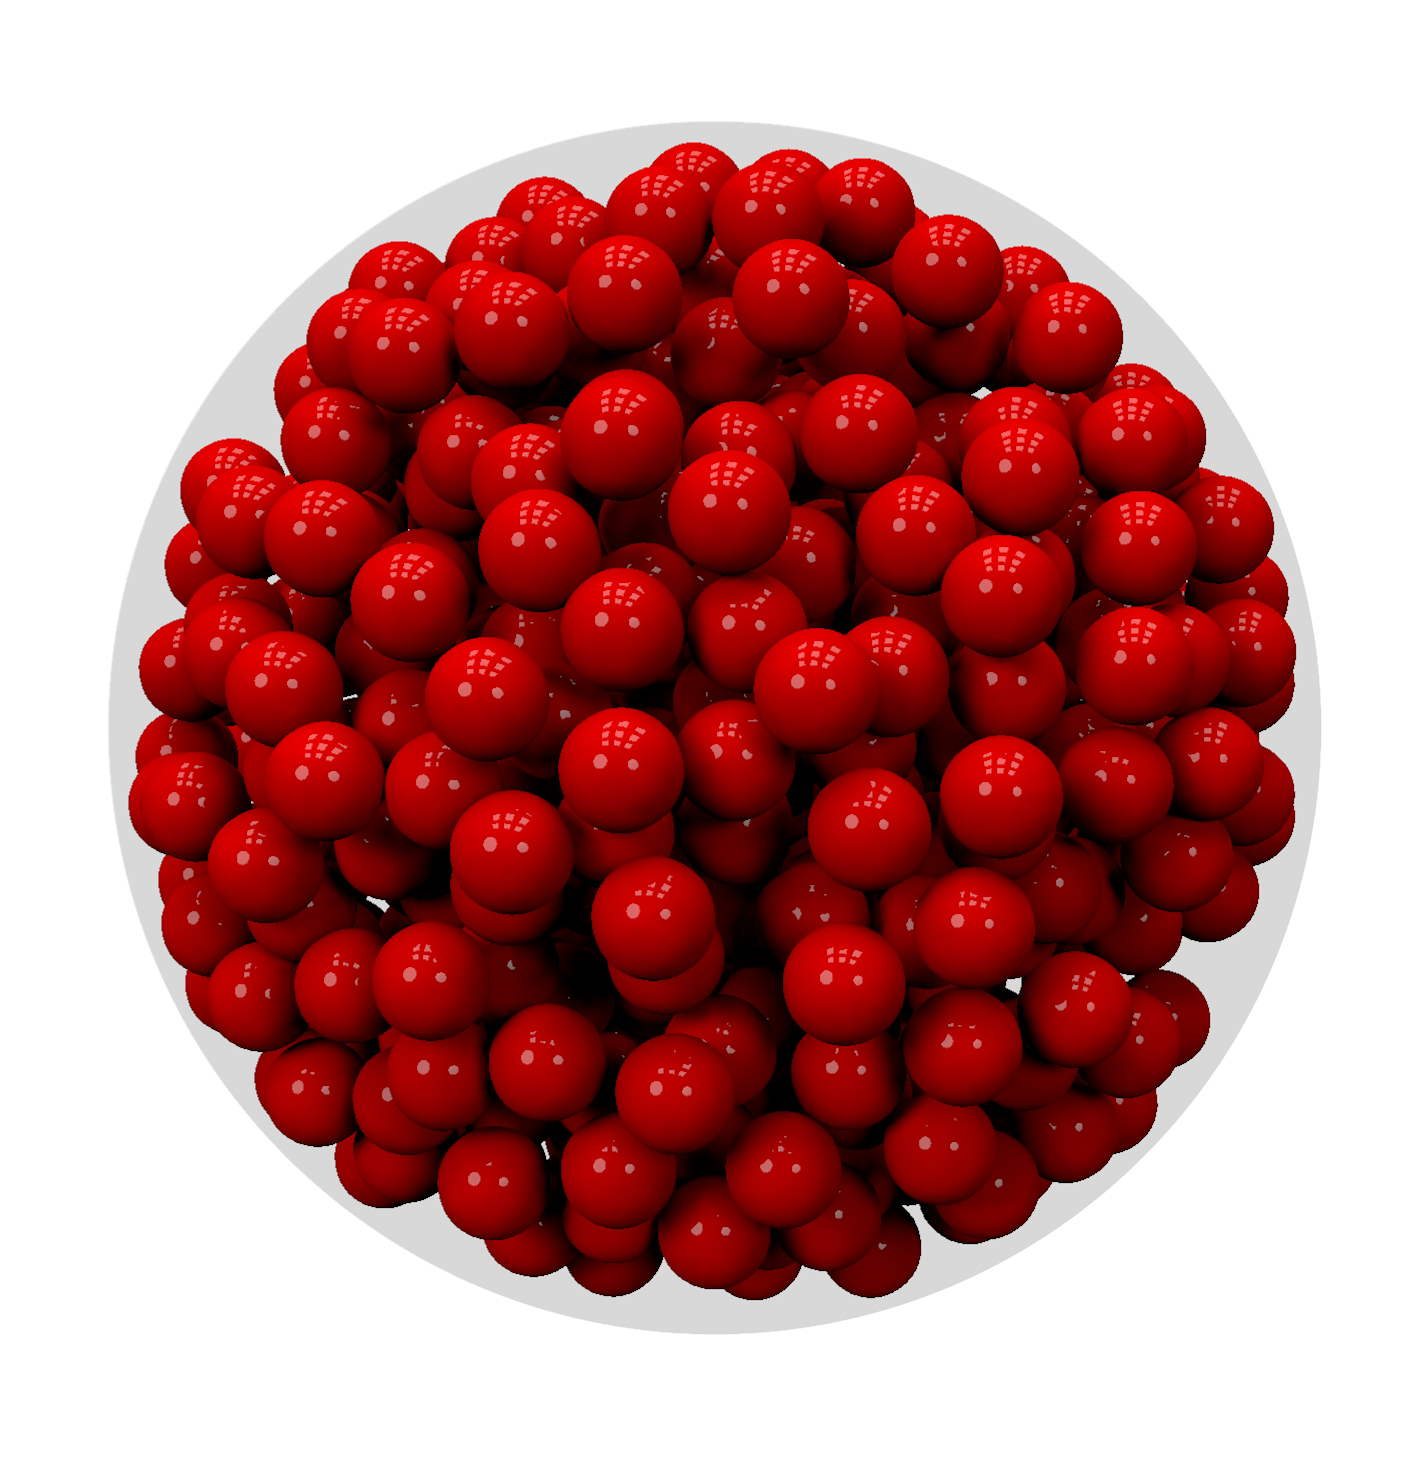
\includegraphics[width=6cm]{chapter_7/figures/fig_1.png} 
\par\end{centering}
\caption{\label{fig:sketch}Representation of the system under study. The centres of the red spheres represent the particles position. The radius of each sphere equals half the L-J potential equilibrium distance $r_{m}/2$. The translucid sphere represents the confining sphere.}
\end{figure}
Here, unless otherwise specified, we consider $515$ particles as can be seen in the sketch of Fig. (\ref{fig:sketch}). In this figure, the particles are represented by a spheres of radius $r_{m}/2$, and the translucid sphere represents the confining spherical volume. In an infinite FCC lattice the maximum filling fraction is $\phi_{\infty}\simeq74\%$. In the case studied, we reach $\phi\approx56\%$. In the process of the generation of the structure, we imposed a condition that only particles inside of the sphere are considered (note that the particles are point particles). This condition gives rise to a reduction of the maximum filling fraction because inaccessible spaces appear along the confining geometry.\\
In order to generate a suitable statistical ensemble at fixed temperature, we perform DMC simulations using the canonical ensemble. We depart from a relaxed structure with energy $E_{i}$. A particle of the ensemble is randomly chosen and it is moved to a new position. This new position, randomly selected, is inside of a sphere with radius $\tilde{r}$ and centred in the previous position of the particle. If the new position is inside the confining sphere,
%and is not a position already occupied by other particle, 
the new position is a valid position to be considered. Otherwise the particle is replaced in the previous position and the calculation returns to the beginning.  At this point, we re-evaluate the system's energy $E_{f}$. The system changes its configuration from one energy to the other with probability $p = e^{-\frac{E_{f}-E_{i}}{T}}$, where $T$ is a control parameter analog to the temperature.\\
If $E_{f} < E_{i}$, the probability is $p = 1$ and the new position is accepted. A direct consequence is the decrease of the total energy of the system. If $E_{f} \geq E_{i}$ the probability of acceptance the new position is smaller than $1$. We generate a random number between the interval $\left[0,1\right]$ and we compare with $p$. If the random number is bigger than $p$, the position is refused, otherwise is accepted. We should note that the "acceptance rate" is controlled by the temperature parameter $T$.\\
 If the new position is accepted, $\tilde{r}$ is resized by a factor of $1.01$, otherwise $\tilde{r}$ is resized by a factor of $0.99$. The full set of steps described above is called single-particle MC step.
We start by performing $10^{8}$ of MC steps to thermalise the system, where no information is collected.
After this process an extensive MC sampling is performed ($10^{5}$ configurations, each configuration obtained after $10^{5}$ single-particle MC steps), where structural information is collected and treated.\\
Here the temperatures and energies presented are given in units of the potential well.

\section{Results and discussion\label{chap:chap7_discussion}}

We determine the temperatures of the (isochore) phase transition in the system by considering the specific heat (SH). The SH, or $C_{v}$, is obtained through the fluctuations of the internal energy \cite{Wang:2001jk}:

\begin{equation}
C_{v}\left(T\right)=\frac{\partial U\left(T\right)}{\partial T}=\frac{\left\langle E^{2}\right\rangle -\left\langle E\right\rangle ^{2}}{T^{2}}.
\end{equation}

\begin{figure}[h]
\begin{centering}
\includegraphics[height=11cm,angle=-90]{chapter_7/figures/fig_2.eps} 
\par\end{centering}
\caption{\label{fig:specific_heat}(a) Specific heat as a function of temperature for a confined L-J system with $N=515$ particles. Zooms of the specific heat is represent in the box (b) and (c).}
\end{figure}
Considering the behaviour of the specific heat as a function of temperature, as shown in Fig. (\ref{fig:specific_heat})(a), we observe a high and narrow peak for $T\approx0.5$. This behaviour is assigned to a first order phase transition, where the system exhibits a discontinuity in the first derivative of the free energy with respect to the temperature.
Notice that in the phase transition region we have relevant fluctuations, as can be observed in Fig. (\ref{fig:specific_heat})(b). Also we observe a modification on SH for temperatures between $0.4\lesssim T\lesssim0.5$
(Fig. \ref{fig:specific_heat})(c), this feature in the SH might be attributed to a pre-melting region. Out of this transition, the behaviour of the specific heat is continuous. Very similar results were recently obtained by Bolmatov \textit{et al.}, where were presented experimental an theoretical results of the constant-volume SH for noble gases \cite{bolmatov2013thermodynamic}.\\

In order to better describe the phase transitions in the system, we also estimate the self-diffusion coefficient in the system as a function of the temperature. To do so, the averaged quadratic displacement of particles as a function of the performed MC steps were fitted to a linear law. From the slope of the lines, the diffusion coefficient is extracted, as can be seen in Fig. (\ref{fig:quad_disp}).\\

\begin{figure}[h]
\begin{centering}
\includegraphics[height=11cm,angle=-90]{chapter_7/figures/fig_4_1.eps} 
\par\end{centering}
\caption{\label{fig:quad_disp}Quadratic mean displacement as a function of the MC steps for $T=0.45$ and $T=0.55$. The blue and green line are the linear fit used to extract the diffusion coefficient.}
\end{figure}
In Fig. (\ref{fig:diff_coef_1}) we plot the diffusion coefficient ($D$) as a function of temperature for three different systems with different number of particles and different volumes, but obeying to the condition of maximum filling fraction. We observe that the diffusion coefficient, for this scale, does not depend of the size of the system. \\
Three regions can be identified in Fig. (\ref{fig:diff_coef_1}). In the first region, for normalized temperatures $T\lesssim0.4$, the diffusion is strongly inhibited. This fact is compatible with a pure solid phase. The diffusion coefficient grows with temperature at an approximately constant rate in the range $0.4\lesssim T\lesssim0.5$
(See Fig. \ref{fig:diff_coef_1})(b). This apparent increase in $D$ signals a pre-meting phase. It is worth noticing that this region does not correspond to any remarkable feature in the specific heat. The slope of the diffusion constant shows a strong increase at about $T\simeq0.5$, this kink in the diffusion coefficient curve corresponds to the peak in the specific heat.\\
In summary, we can establish a phase landscape in which, we identify a pre-melting region that starts at $T\simeq0.4$, and a (solid-liquid) phase transition at $T\simeq0.5$.

\begin{figure}[h]
\begin{centering}
\includegraphics[height=10cm, angle=-90]{chapter_7/figures/fig_3.eps} 
\par\end{centering}
\caption{(a) Diffusion coefficient as a function of the temperature, for three different system sizes of the system at constant particle density. (b) Zoom of the same plot in the range $0.15<T<0.75$.\label{fig:diff_coef_1}}
\end{figure}
In Fig. (\ref{fig:chap7_energy_fluctuations}) we represent the particle energy as a function of the MC steps for temperature $T=0.53625$, which corresponds to a temperature in the phase transition region. The system at this temperature oscillates between a lower and a higher value of energy. This bistable energy behaviour is the responsible for the fluctuations in the SH. Despite the large number of MC steps used in the sampling, we observe in Fig. (\ref{fig:chap7_energy_fluctuations}) that the number of high and low energy regions is relatively reduced. Hence, if we calculate the SH through the energy fluctuations of internal energy, large fluctuations due to finite sampling is expected, as observed in Fig. (\ref{fig:specific_heat})(b).

\begin{figure}[h!]
\begin{centering}
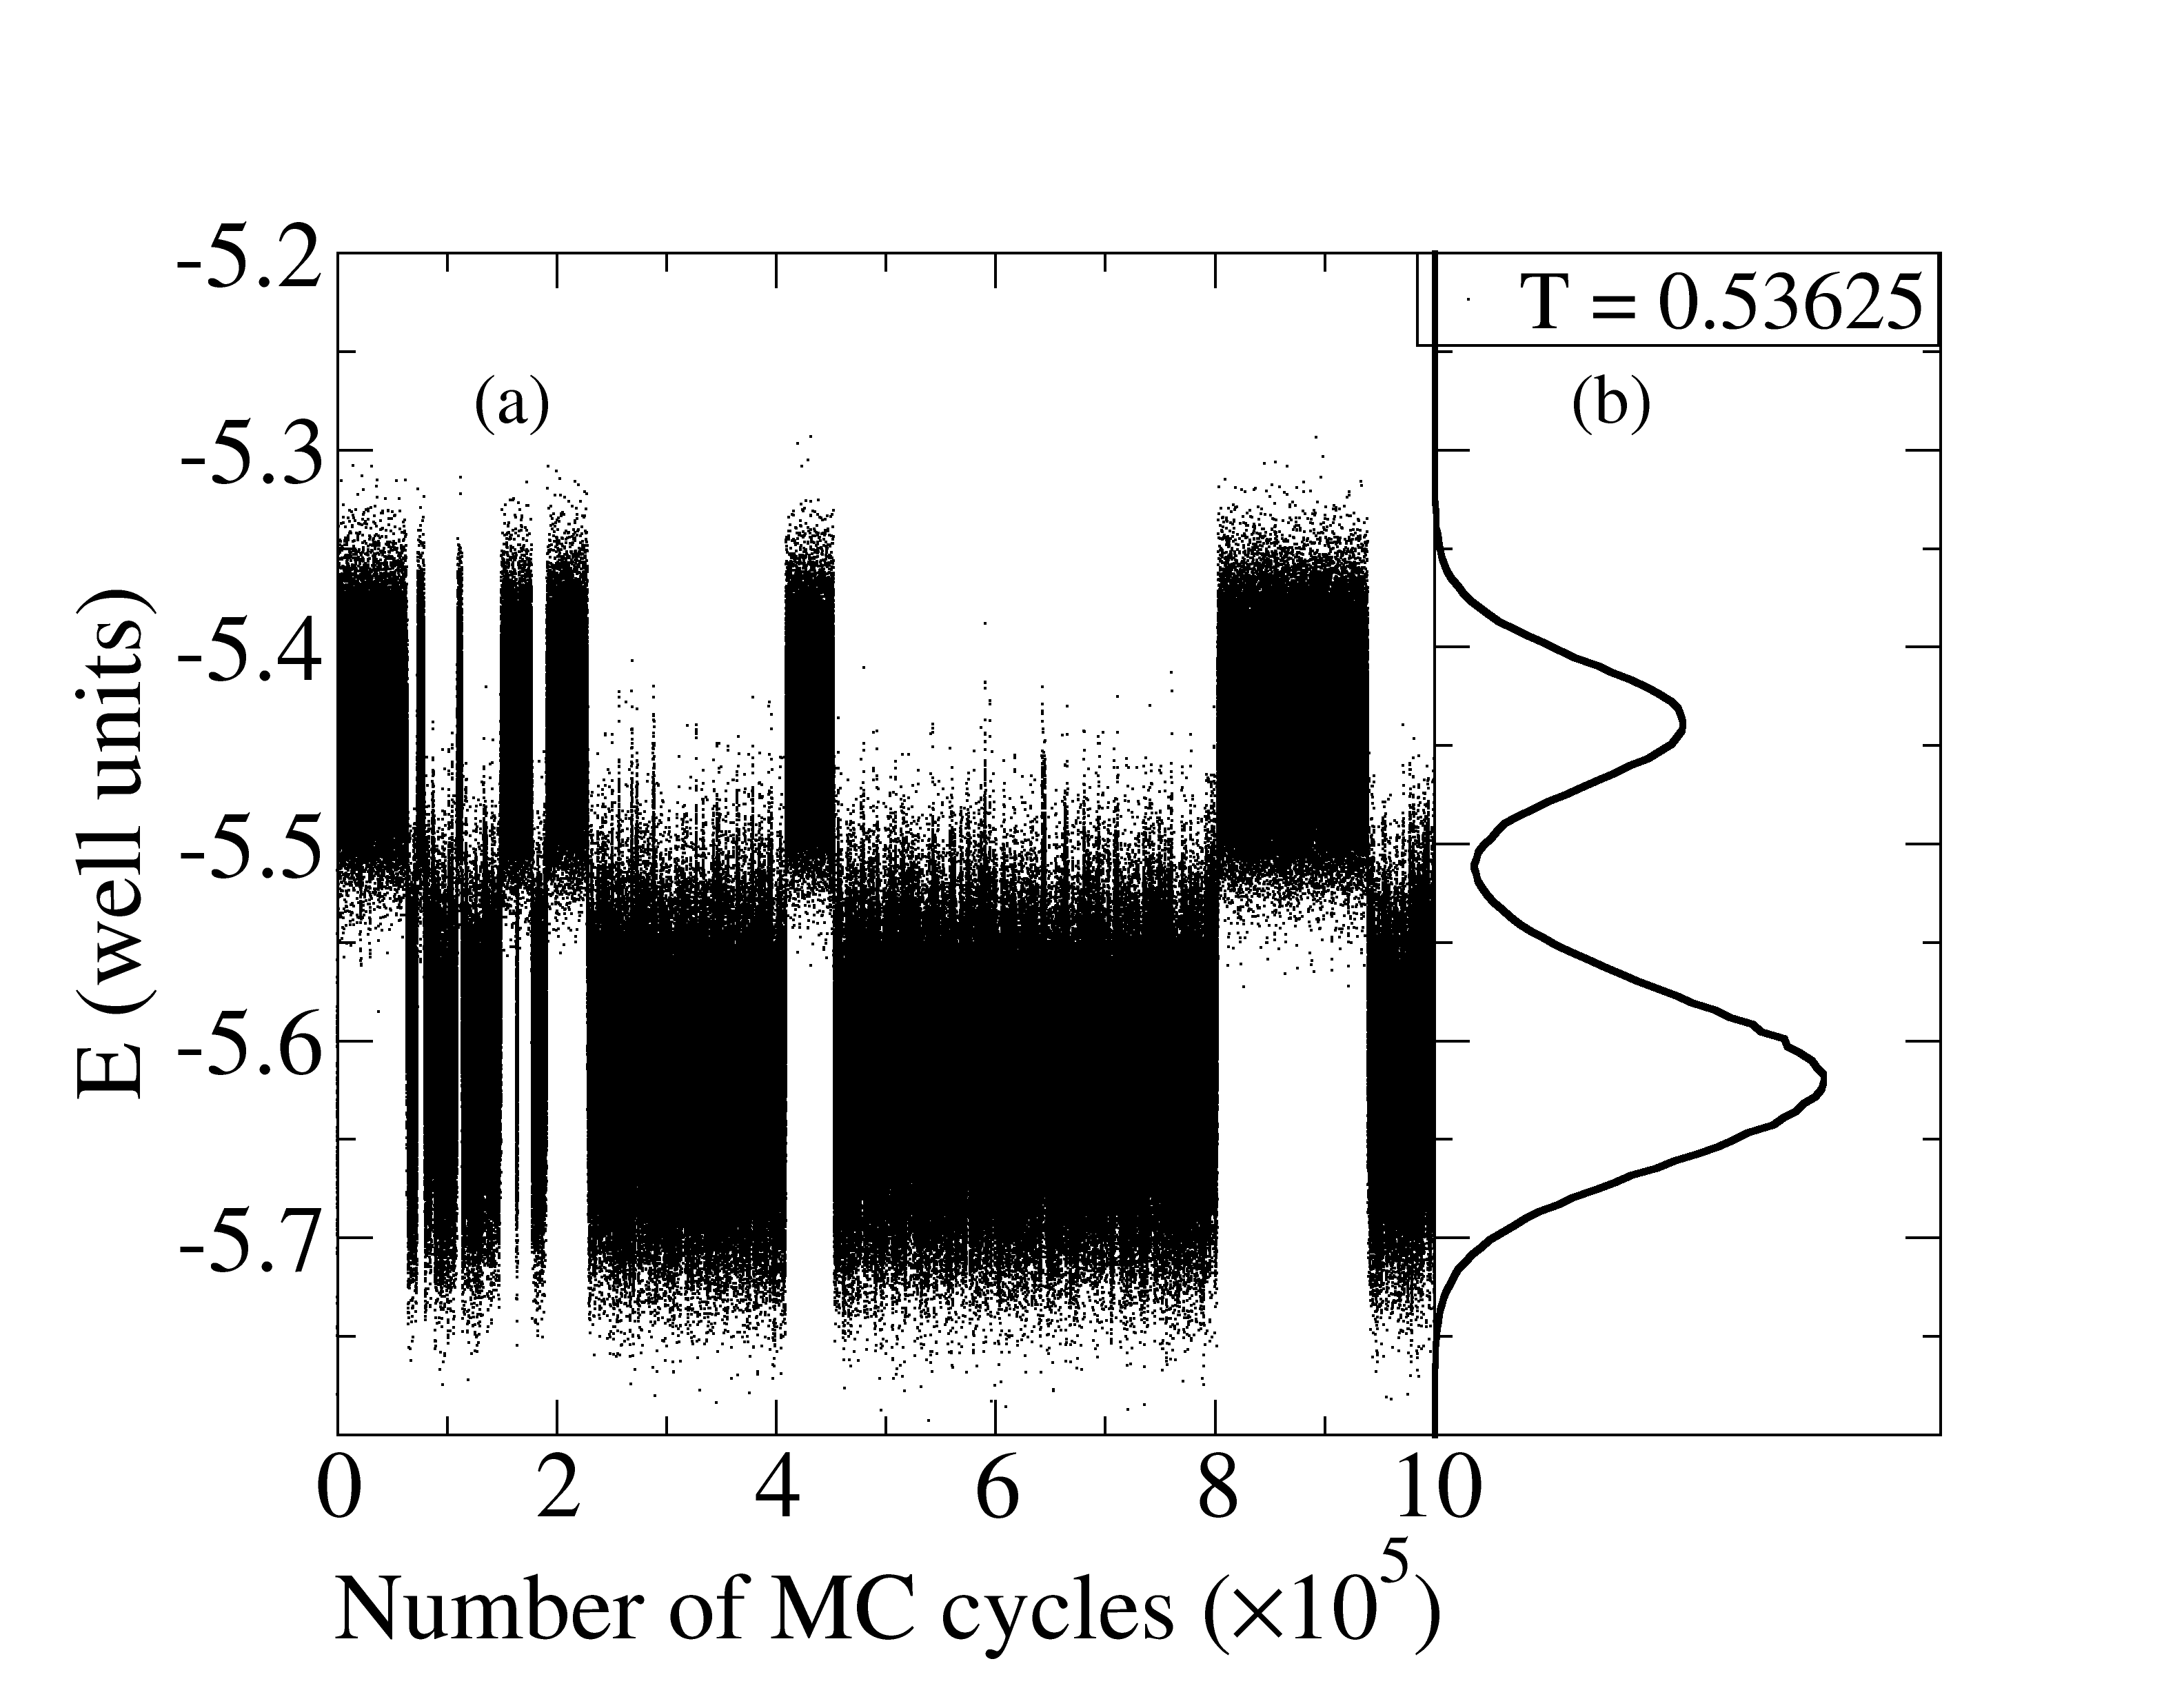
\includegraphics[height=9cm]{chapter_7/figures/fig_4.png}
\par\end{centering}
\caption{\label{fig:chap7_energy_fluctuations} (a) Energy sampling of a confined L-J system during a full MC run at a temperature $T=0.53625$, corresponding to a phase-switching region. (b) Energy histogram obtained from the MC sampling in (a). }
\end{figure}
Representing the internal energy histogram as a function of the temperature, shown in Fig. (\ref{fig:colormap_distrib}), we can identify an energy gap for temperatures at the phase transition. The transition between solid and liquid is not smooth with phase coexistence between two states. Instead, the system switches between this two phases, with abrupt modifications in a small number of MC cycles. In the phase transition, when the particles exhibit a low energy configuration, the system is in the solid phase. For higher energies, the system is in the liquid phase. Interestingly, phase coexistence, that might be attributed to intermediate energies in the energy histogram, appear with very low probability as a gap in the distribution.\\
\begin{figure}[h]
\begin{centering}
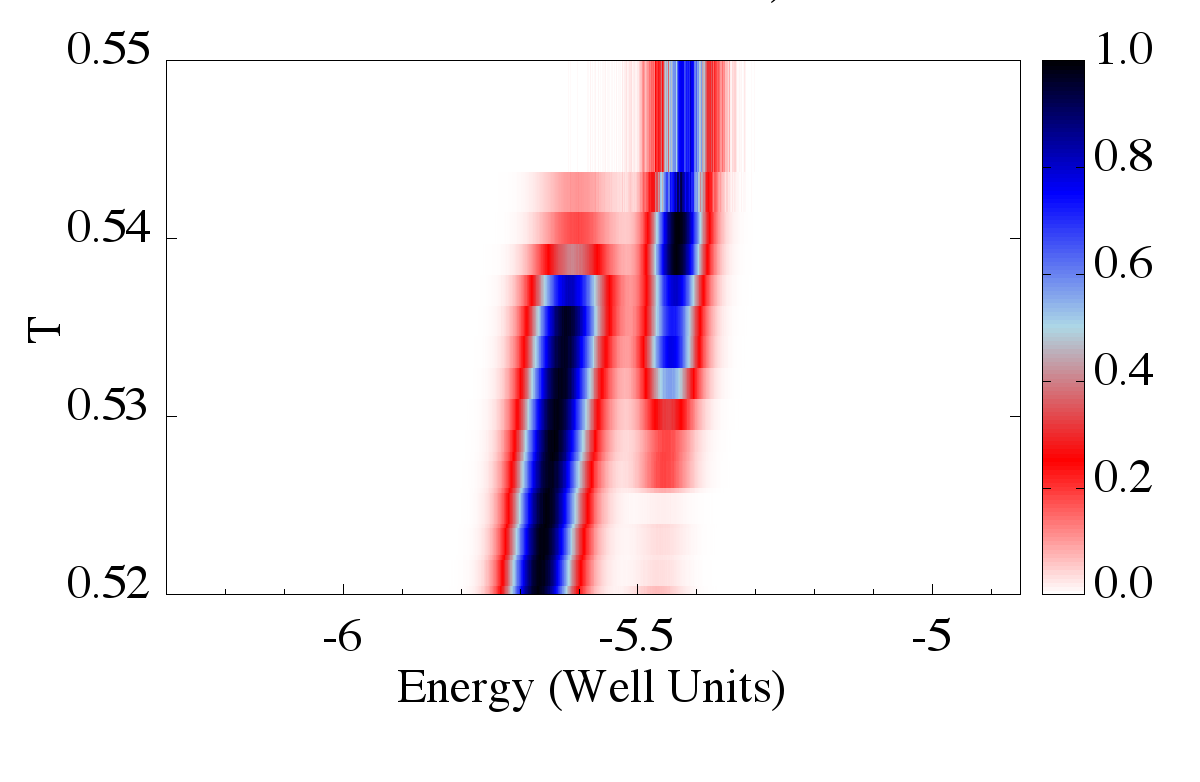
\includegraphics[height=11cm]{chapter_7/figures/fig_5.png} 
\par\end{centering}
\centering{}\caption{(a) Colormap showing the energy distribution functions as a function of the temperature. (b) Zoom in the region corresponding to the solid-liquid phase transition.\label{fig:colormap_distrib}}
\end{figure}
In order to better understand the geometrical and dynamical properties of the system in the phase switching region, we observe that the system remains in either the lower or the upper energy branches for a sufficient amount of time (MC steps) to consider both the structural (pair correlation function) or dynamical (self-diffusion constant) properties in well defined phases.\\
Regarding dynamical properties, in Fig. (\ref{fig:massive_diffusion_coef})(c) we plot the self-diffusion constant as a function of temperature much in the same way as done in Fig. (\ref{fig:diff_coef_1}). In this case, we have split the statistical ensemble in two different sets for temperatures in the phase switching region, one corresponding to the high energy branch (liquid phase), and the other one corresponding to lower energy branch (solid phase). In Fig. (\ref{fig:massive_diffusion_coef})(c) it appears evident that the diffusion coefficients corresponding to both phases can differ by a large amount. In the case under study, the diffusion constant differs by a factor 3 between phases at the same temperature.\\

\begin{figure}[h]
\begin{centering}
\includegraphics[height=10cm, angle=-90]{chapter_7/figures/fig_6.eps} 
\par\end{centering}
\caption{\label{fig:massive_diffusion_coef}(a) Self-diffusion coefficient for a 515 particle system as a function of temperature. (b) Zoom of the self-diffusion coefficient in the range $0.35\leq T\leq0.6$. (c) Self-diffusion coefficients as a function of temperature obtained for the liquid phase (upper branch) and the solid phase (lower branch) in the region of phase-switching.}
\end{figure}
Regarding geometrical properties of both phases in the phase switching region, we have studied the radial distribution function $g\left(r\right)$ \cite{Percus:1958wv,Wertheim:1963tb}. This function is defined as the ratio of the average number density at a distance $r$ from one particle to the averaged number density of an hypothetical, fully uncorrelated, system (see Appendix \ref{App:Radial_distribution_function}). Hence, the radial distribution function describes the correlation in the inter-particle distance in the system. Again, we can split the statistical sampling in two sets associated with upper and lower energy branches in the phase switching region.\\
Contrary to what intuition might suggest, and in contrast with the behaviour of the diffusion constants, the radial distribution function in the upper and lower energy branches is very similar. In Fig. (\ref{fig:chap7_Radial-distribution-function}) we represent the $g\left(r\right)$ for the configurations at both the liquid and solid phase at a fixed temperature.\\
In the solid phase, the structure of the radial distribution function (black line in Fig. (\ref{fig:chap7_Radial-distribution-function})) shows a slightly richer structure than the one corresponding to the liquid phase (red line in Fig. (\ref{fig:chap7_Radial-distribution-function})). Nevertheless, both curves differ by less than 10\% in its values in the whole range of temperatures of the phase switching region, in contrast with the large variations observed in the self-diffusion coefficients. This fact suggests that, despite the subtle peak suppression in $g\left(r\right)$ in the in the switching from solid to liquid phases, a clear identification of different phases through structural measurements (\textit{eg.} radial distribution function) is less sensitive than through dynamical measurements (\textit{eg.} self-diffusion constants) in strongly confined systems. 

\begin{figure}[H]
\begin{centering}
\includegraphics[height=11cm, angle=-90,clip=true]{chapter_7/figures/fig_7.eps} 
\par\end{centering}
\caption{\label{fig:chap7_Radial-distribution-function}Radial distribution function $g\left(r\right)$ obtained at a fixed temperature in the phase switching region ($T=0.53625$) for both the solid (black line) and liquid (red line) phases. }
\end{figure}

\section{Conclusion\label{chap:chap7_conclusions}}

In this chapter we have studied the self-diffusion in a strongly confined Lennard-Jones system. For small clusters, of the order of a few hundreds of particles, instead of phase coexistence, like in macroscopic systems, the system present dynamic phase switching between solid-like and liquid-like phases. This was concluded from monitoring the energy as a function of the system evolution, where the system oscillates between an high energy and a low energy configuration.\\
We found that the self-diffusion coefficient of the liquid-like phase in the phase-switching region can be up to a factor of three larger than the one associated to the solid phase. Surprisingly, the radial distribution function of the liquid and solid phases are essentially indistinguishable. Our results strongly suggest that retrieving relevant information in a system undergoing phase switching involve measurements either of the internal energy evolution or the self-diffusion characteristics of the system. Structural information does not provide a relevant signature of phase switching in this case.\\
In the next chapter we shall study the implications of the behaviour of this system on the optical transport and emission properties.





